\documentclass[12pt]{article}
\usepackage[margin=1in]{geometry}
\usepackage{alltt}
\usepackage{subfig}
\usepackage{epsfig}
\usepackage{hyperref}
\usepackage{setspace}
\usepackage{gensymb}
\usepackage{libertine} 
\usepackage{siunitx}
\usepackage{amsmath}
\usepackage{placeins}
\usepackage{enumitem}
\newlist{steps}{enumerate}{1}
\setlist[steps, 1]{label = Step \arabic*:}
\usepackage{indentfirst}
\usepackage{float}
\usepackage{lscape}
\usepackage[blocks]{authblk}
\doublespacing
\renewcommand{\baselinestretch}{1}
\setlength{\textheight}{9in}
\setlength{\textwidth}{6.5in}
\setlength{\headheight}{0in}
\setlength{\headsep}{0in}
\setlength{\topmargin}{0in}
\setlength{\oddsidemargin}{0in}
\setlength{\evensidemargin}{0in}
\setlength{\parindent}{.3in}
%%%%%%%%%%%%%%%%%%%%%%%%%%%%%%%%%%%%%%%%%%%%%%%%%%%%%%%%%%%%%%%%%%%%%%
\begin{document}
\input{title_page_1}
\newpage
%%%%%%%%%%%%%%%%%%%%%%%%%%%%%%%%%%%%%%%%%%%%%%%%%%%%%%%%%%%%%%%%%%%%%%%%%%%%%%%%%%%%%%%%%%%%%%
\section*{Abstract}
\begin{doublespace}
The purpose of this design project was to perform a dynamic simulation of the four-bar windshield wiper mechanism driven by the AM equipment 328 gear motor. Several methods were employed to describe the dynamic response of the mechanism. These processes were in terms of {\tt MATLAB} functions. These include the vector loop method, Newton's method, basic $1^{st}$ and $2^{nd}$ order kinematic coefficient, the power equation, the load torque, the driving torque, and the Euler method function. The end result from this dynamic simulation include the dynamic response of $\dot{\theta}_{2}$ vs. time, $\dot{\theta}_{5}$ vs. time, fluctuation coefficient at steady State, time required for a clean windshield, and the maximum load of wiper. Values for the fluctuation coefficient, time required, and the maximum wiper load were $C_{f} = 6.13 \%$, $t_{req} = 1.83 \quad (seconds)$, $T_{max} = 19.97 \quad (ft lb_{f})$, respectively. These results are discussed in the following section, namely the {\bf Engineering Analysis}.
\end{doublespace}
%%%%%%%%%%%%%%%%%%%%%%%%%%%%%%%%%%%%%%%%%%%%%%%%%%%%%%%%%%%%%%%%%%%%%%%%%%%%%%%%%%%%%%%%%%
\section*{Engineering Analysis - Dynamic Analysis for Four-Bar Windshield Wiper Mechanism}
\begin{doublespace}
As described in the {\bf Abstract}, the windshield wiper mechanism consists of a four-bar mechanism driven by an AM Equipment gear motor. Essentially, this mechanism's gear motor rotates link 2 continuously similar to a crank which causes link 4 to oscillate like a rocker. Gear 3 drives gear 5 which oscillates the wiper of nearly $180^{\degree}$. Figure (\ref{xx1}) describes the windshield wiper schematically. To understand and obtain the dynamic analysis of this wiper mechanism it is necessary to provide an illustration of the process. Figure(\ref{x1}) outlines an engineering analysis for determining the $\dot{\theta}_{2}$ vs. time, $\dot{\theta}_{5}$ vs. time, fluctuation coefficient, time required, and the maximum load of wiper. This concept was done using multiple functions to systematically and routinely compute the desired terms.
\end{doublespace}
%%%%%%%%%%%%%%%%%%%%%%%%%%%%%%%%%%%%%%%%%%%%%%%%%%%%%%%%%%%%%%%%%%%%%%%%%%%%%%%%%%%%%%%%%%%
  \begin{figure}[H]
  \begin{center}
  $\begin{array}{c}
  \includegraphics[width=4.5in]{rolling1.png} 
  \end{array}$
  \end{center}
  \caption{Free body diagram of the AM equipment 238 and its links associated links}
  \label{xx1}
  \end{figure}
%%%%%%%%%%%%%%%%%%%%%%%%%%%%%%%%%%%%%%%%%%%%%%%%%%%%%%%%%%%%%%%%%%%%%%%%%%%%%%%%%%%%%%%%%%%
  \begin{figure}[H]
  \begin{center}
  $\begin{array}{c}
  \includegraphics[width=4.5in]{rolling2.png}
  \end{array}$
  \end{center}
  \caption{The kinematics of AM equipment 238 illustrating its configuration of emotion}
  \label{xx2}
  \end{figure}
%%%%%%%%%%%%%%%%%%%%%%%%%%%%%%%%%%%%%%%%%%%%%%%%%%%%%%%%%%%%%%%%%%%%%%%%%%%%%%%%%%%%%%%%%%%
  \begin{figure}[H]
  \begin{center}
  $\begin{array}{c}
  \includegraphics[width=6.5in]{flowchart3.pdf} %Just take snapshot
  \end{array}$
  \end{center}
  \caption{Flowchart for computing coefficient of fluctuation, time required, and the maximum load of wiper, where $(*)$ indicates detailed information within the Appendix}
  \label{x1}
  \end{figure}
%%%%%%%%%%%%%%%%%%%%%%%%%%%%%%%%%%%%%%%%%%%%%%%%%%%%%%%%%%%%%%%%%%%%%%%%%%%%%%%%%%%%%%%%%%%%
\begin{doublespace}
Figure (\ref{xx2}) shows the vector loop with link lengths $\vec{r}_{1},\vec{r}_{2},\vec{r}_{3},\vec{r}_{4}$ defining the four-bar mechanism. Vector $\vec{r}_{5}$ is attached to gear 5 and defines the direction of the windshield wiper blade which rotates
with 5. Figure (\ref{xx2}) also shows the assembly configuration where the initial values ${{\theta}_{3}}_{i}$, ${{\theta}_{4}}_{i}$, and ${{\theta}_{5}}_{i}$ are defined. The assembly configuration corresponds to when the four bar mechanism portion is in a limit position ${{}\dot{\theta}_{5}}_{i} = 168.5^{\degree}$ and the windshield wiper is horizontal. The vector loop equation is:
\end{doublespace}
\begin{eqnarray*}
	\vec{r}_{2} + \vec{r}_{3} - \vec{r}_{4} - \vec{r}_{1} = \vec{0}
\end{eqnarray*}
The scalar components of this mechanism are:
\begin{eqnarray}
	{r}_{2}\cos(\theta_{2}) + {r}_{3}\cos(\theta_{3}) - {r}_{4}\cos(\theta_{4}) - {r}_{1} = 0 \label{ee}
\end{eqnarray}
\begin{eqnarray}
	{r}_{2}\sin(\theta_{2}) + {r}_{3}\sin(\theta_{3}) - {r}_{4}\sin(\theta_{4}) = 0 \label{e1}
\end{eqnarray}
Since there is only one rolling contact between the gears, the rolling contact equation is:
\begin{eqnarray*}
	\rho_{5}\Delta\theta_{5/4} = -\rho_{3}\Delta\theta_{3/4}
\end{eqnarray*}
In this mechanism $\rho_{5}$ = $\rho_{3}$, which simplifies the rolling contact equation to:
\begin{eqnarray*}
	\Delta\theta_{5/4} = -\Delta\theta_{3/4} \rightarrow \Delta\theta_{5}-\Delta\theta_{4} = -(\Delta\theta_{3} - \Delta\theta_{4}) \rightarrow \Delta\theta_{5} - 2\Delta\theta_{4} + \Delta\theta_{3} = 0
\end{eqnarray*}
\begin{eqnarray}
	(\theta_{5}-\theta_{5_i}) - 2(\theta_{4}-\theta_{4_i}) + (\theta_{3}-\theta_{3_i}) = 0 \label{e2}
\end{eqnarray}
\begin{doublespace}
 Equations (\ref{ee})-(\ref{e2}) are a system of three position equations. The scalar knowns in this mechanism are: $\theta_{5_i} = 174^{\degree}$, $\theta_{4_i} = 221^{\degree}$, $\theta_{3_i} = 348^{\degree}$, $\theta_{1} = 0^{\degree}$, ${r}_{1} = 5.625$in., ${r}_{2} = 0.75$in., ${r}_{3} = 5.625$in., ${r}_{4} = 1.3$in., ${r}_{5} = 2$ft. The scalar unknowns for this mechanism are: $\theta_{2}$, $\theta_{3}$, $\theta_{4}$, and $\theta_{5}$. Three position equations with four unknowns means that this mechanism has one degree of freedom. Since $\theta_{2}$ is the input variable, its possible to make a guess in order to obtain $\theta_{3}$, $\theta_{4}$, and $\theta_{5}$.
 \end{doublespace}
%%%%%%%%%%%%%%%%%%%%%%%%%%%%%%%%%%%%%%%%%%%%%%%%%%%%%%%%%%%%%%%%%%%%%%%%%%%%%%%%%%%%%%%%%%%%
\section*{Results - Dynamic Analysis for Four-Bar Windshield Wiper Mechanism}
\begin{doublespace}
This section provides the plots of $\dot{\theta}_{2}$ vs $time$, $\dot{\theta}_{5}$ vs $time$, as well as the fluctuation coefficient at steady State, the time required for a clean windshield, and the maximum load of wiper. \\ 
\indent
The values for the coefficient of fluctuation, time required, and the maximum wiper load were $C_{f} = 6.13 \%$, $t_{req} = 1.83 \quad (seconds)$, $T_{max} = 19.97 \quad (ft lb_{f})$, respectively. According to Figure (\ref{x3}), the dynamic simulation shows that steady state is reached at about $t_{req} = 1.83 (seconds)$. At the same moment, in Figure (\ref{x2}) the crank speed oscillates between a maximum of ${{}\dot{\theta}_{2}}_{max} = 33.85 (rpm)$, a minimum of ${{}\dot{\theta}_{2}}_{min} = 31.84 (rpm)$, and an average of ${{}\dot{\theta}_{2}}_{avg} = 32.85 (rpm)$. Evidently, all these values correspond to positive crank velocities because the rotation in this case is counter-clockwise. The steady state speed variation of a machine determined by the coefficient of fluctuation. Here the coefficient of fluctuation is not too extreme. This is desirable since higher fluctuations in the crank speed at steady state leads to extreme operation factors. A few examples of these extremities are large bearing forces, large loading on the motor, and heat due to repeated motor slip. There were multiple prerequisites in order to obtain the dynamic response for this mechanism. One of which was to use Newton's method along with it's vector loop equation. In order to employ Newton's method, one must be able to solve the vector loop equation and take its first $x$ and $y$ component derivatives with respect to the input $\theta_{2}$. The scalar knowns and unknowns were also given to mimic the windshield wiper's response. All relevant information including the complete windshield wiper mechanism can be viewed in {\bf Appendix B}. {\bf Appendix A} identifies a detailed description of the windshield wiper mechanism as well as the gear motor used. This information is critical in order to compute the Basic $1^{st}$ and $2^{nd}$ order Kinematic Coefficient of $h_{3}$, $h_{4}$, $h_{5}$, and $h^{\prime}_{3}$, $h^{\prime}_{4}$, $h^{\prime}_{5}$ with respect to $S_{i} = \theta_{2}$. {\bf Appendix C} to compute the Kinetic Energy for the A terms, B terms and their individual sums, $\sum A$'s and $\sum B$'s. These definitions represent the collection of moving parts within a machine. To obtain this result, the Power Equation in equation will be reduced to only a term representing the rate change in kinetic energy. This is by assuming that at lower inertias and high speeds, kinetic energy tends to dominate potential energy and the power dissipated through friction. Thus, both terms in the power equation can be ignored. After defining the $1^{st}$ and $2^{nd}$ order Kinematic Coefficient and their mass centers, the kinetic energy can be differentiated to obtain the final result on equation (7.5). The inertias considered in this design set are the Wiper Blade, Motor Windings, Worm Gear, and Worm Wheel. These parts are moving within a machine. Therefore, they each have a $1^{st}$ and $2^{nd}$ order Kinematic Coefficient and their mass centers. {\bf Appendix D} describes how the load torque is computed for a given $\theta_{2}$ value. This is done by knowing that the windshield wiper oscillates clockwise to remove the debris from the windshield and counter clock wise to reset the wiper back to its original position. {\bf Appendix E} demonstrates how the driving torque is calculated by finding $T_{stall}$ and the maximum angular velocity of the motor at low speeds on {\bf Appendix A} and also knowing that ${{}\dot{\theta}_{2}}$ is constant throughout the motion the wiper. Finally, {\bf Appendix E} determines ${{}\dot{\theta}_{5}}$, $\delta{\theta_{2}}$, $\delta{t}$, and $\delta{{}\dot{\theta}_{2}}$ in order to successfully compute the solution of the forward dynamics problem such that the loop cycles and iterates for a value of $\theta_{2}$. 
\end{doublespace}
%%%%%%%%%%%%%%%%%%%%%%%%%%%%%%%%%%%%%%%%%%%%%%%%%%%%%%%%%%%%%%%%%%%%%%%%%%%%%%%%%%%%%%%%%%%%
  \begin{landscape}
  \begin{figure}[H]
  \begin{center}
  $\begin{array}{c}
  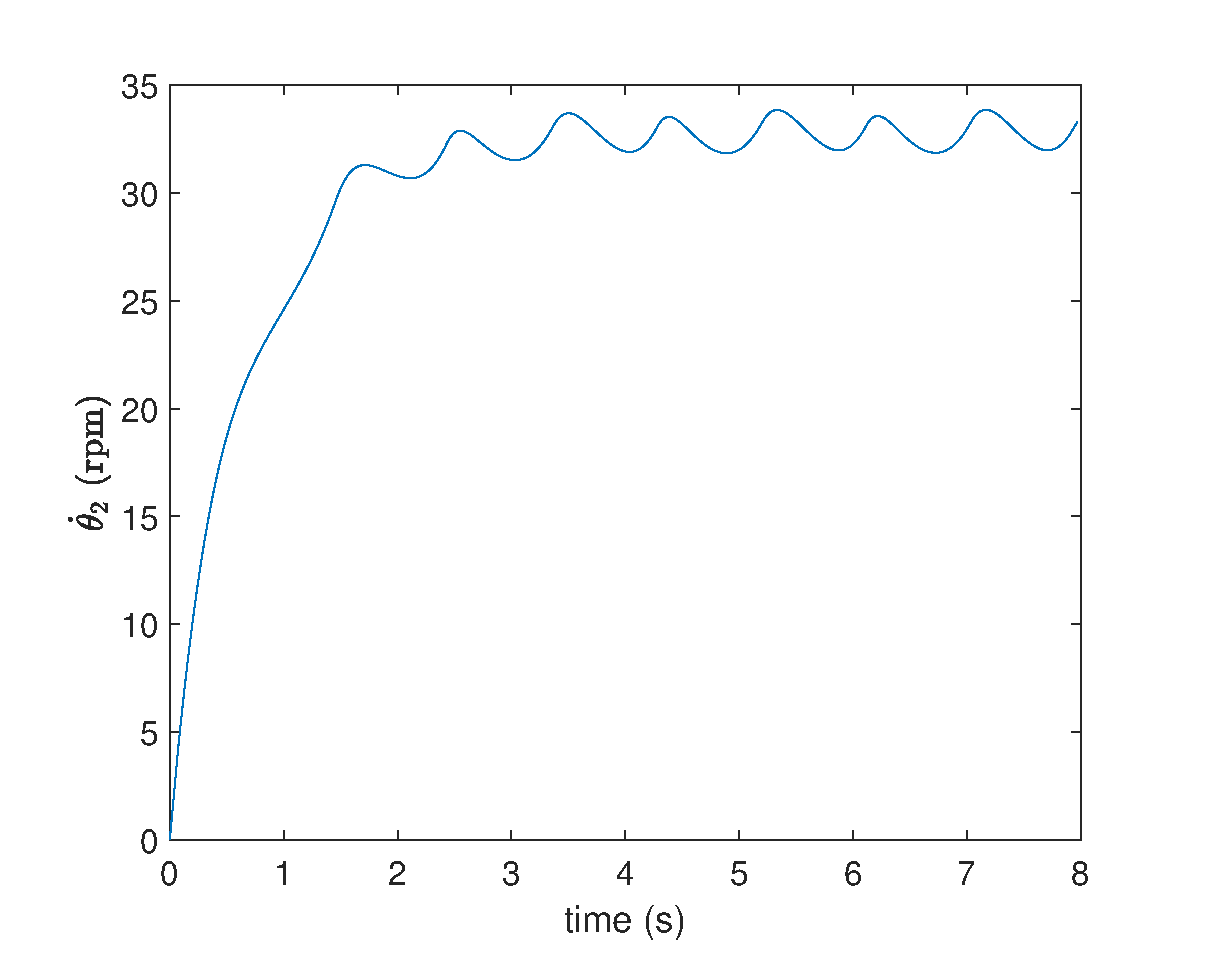
\includegraphics[width=5in]{figure13.eps}
  \end{array}$
  \end{center}
  \caption{Graphical representation of an Inverse Dynamics Problem applied to motor selection AM238 Series gearmotor outputing $\dot{\theta_2}$ revolutions per minute with increasing time in seconds}
  \label{x2}
  \end{figure}
  \end{landscape}
  %%%%%%%%%%%%%%%%%%%%%%%%%%%%%%%%%%%%%%%%%%%%%%%%%%%%%%%%%%%%%%%%%%%%%%%%%%%%%%%%%%%%%%%%%%%%%
  \newpage
  %%%%%%%%%%%%%%%%%%%%%%%%%%%%%%%%%%%%%%%%%%%%%%%%%%%%%%%%%%%%%%%%%%%%%%%%%%%%%%%%%%%%%%%%%%%
  \begin{landscape}
  \begin{figure}[H]
  \begin{center}
  $\begin{array}{c}
  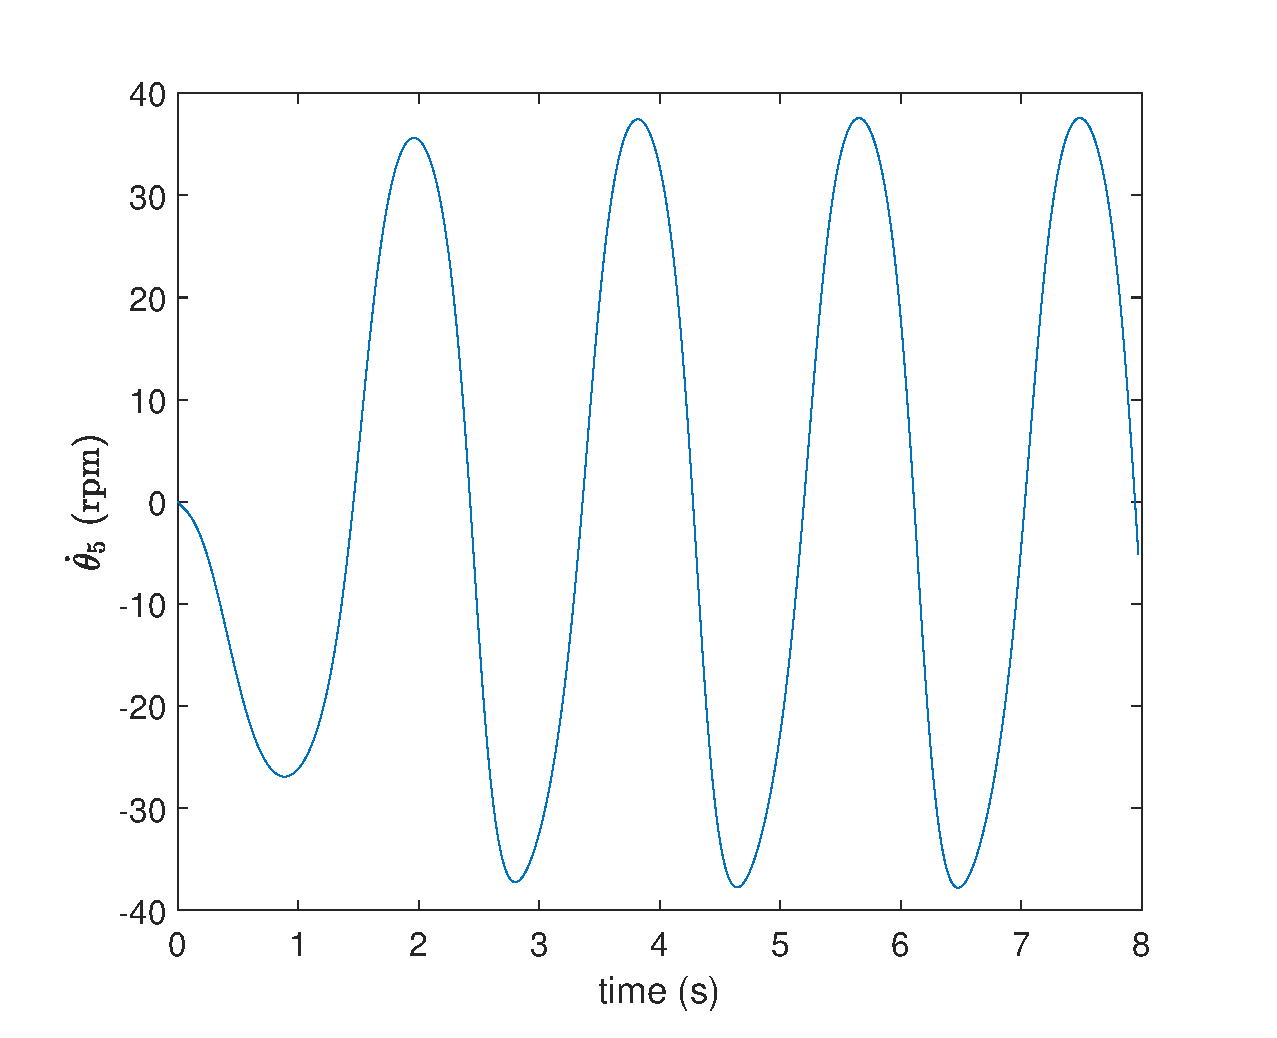
\includegraphics[width=5in]{figure14.eps}
  \end{array}$
  \end{center}
  \caption{Describing the velocity rate of change of joint variable $\dot{\theta_5}$ in revolutions per minute while increasing time in seconds}
  \label{x3}
  \end{figure}
  \end{landscape}
%%%%%%%%%%%%%%%%%%%%%%%%%%%%%%%%%%%%%%%%%%%%%%%%%%%%%%%%%%%%%%%%%%%%%%%%%%%%%%%%%%%%%%%%%%%%%
\section*{Appendix A}
\begin{doublespace}
This section describes the dynamic simulation and motor selection for the four-bar windshield wiper mechanism. As previously mentioned, to determine the dynamic response of the system, it is necessary to analyze the links of the 4-bar mechanism, its scalar components, the rolling contact equation, and the mechanism's scalar knows and unknowns. The following reference specifies the information page and the conversion table for the AM Equipment 238 gearmotor. The information presented in this gearmotor provide an output torque as a function of the angular velocity, and the gear ratio of the worm gear drive of $83:1$.

% \begin{verbatim}

% \end{verbatim}
\end{doublespace}
\newpage
%%%%%%%%%%%%%%%%%%%%%%%%%%%%%%%%%%%%%%%%%%%%%%%%%%%%%%%%%%%%%%%%%%%%%%%%%%%%%%%%%%%%%%%%%%%%
\section*{Appendix B: Newton's Method}
\begin{doublespace}
This section gathers the initial values from the input section of the design project and computes values of $\theta_{3}$, $\theta_{4}$, and $\theta_{5}$ for a value of $\theta_{2}$.
\end{doublespace}

\begingroup
\fontsize{8pt}{10pt}\selectfont
\begin{verbatim}
function [t3r,t4r,t5r]= nmet4matrixmult(r1,r2,r3,r4,t2r,t3r,t4r,t5r,t5ri,t4radi,t3radi)
%%% This program uses the ""Function"" command to call inputs from x_o and 
%%% runs it into the program until the error is less than or equal to 
%%% the tolerance.
%%% This program was used in Programming Problem 2; Its now being implemented in
%%% Design Set 2. 
%%% r1, r2, r3, r4 are all known link lengths (in). 
%%% t2 will be in a range of 0-2pi in terms of radians.

x_o = [t3r;t4r;t5r]; %;t5r] % defining the vector of inital guess which 
                 % will already in radians once the function 
                 % is called in the main program
% setting tolerance for convergence
tol= .1;
% setting initial error greater than tolerance to begin loop
error= 10;
while error>tol
    % setting sines and cosines of angles t2, t3, t4
    st2= sin(t2r);
    ct2= cos(t2r);
    st3= sin(t3r);
    ct3= cos(t3r);
    st4= sin(t4r);
    ct4= cos(t4r);
    f1= r2*ct2+r3*ct3-r4*ct4-r1;   
    f2= r2*st2+r3*st3-r4*st4;
    f3= (t5r-t5ri)-2*(t4r-t4radi)+(t3r-t3radi);
    f= [f1; f2; f3];
    dfdt3= [-r3*st3; r3*ct3; 1];  
    dfdt4= [r4*st4; -r4*ct4; -2]; 
    dfdt5= [0; 0; 1];
    A= [dfdt3,dfdt4,dfdt5];
    x= -pinv(A)*f+ x_o;
    t3r= x(1,1);
    t4r= x(2,1);
    t5r= x(3,1);
    %t5r= 2*(t4r - t4radi) - (t3r - t3radi) + t5ri;
    error = norm(x-x_o);
    x_o=x;
end
end
\end{verbatim}
\endgroup

\newpage

%%%%%%%%%%%%%%%%%%%%%%%%%%%%%%%%%%%%%%%%%%%%%%%%%%%%%%%%%%%%%%%%%%%%%%%%%%%%%%%%%%%%%%%%%%%%
\section*{Appendix C: Basic $1^{st}$ and $2^{nd}$ order Kinematic Coefficent Function}
\begin{doublespace}
This section uses the Newton's Method code to compute $h_{3}$, $h_{4}$, $h_{5}$ and their derivatives, $h^{\prime}_{3}$, $h^{\prime}_{4}$, and $h^{\prime}_{5}$.
\end{doublespace}

\begingroup
\fontsize{8pt}{10pt}\selectfont
\begin{verbatim}
function [f_g5xp, f_g5yp, h5p, h4p, h3p, f_g5y, f_g5x, h5, h4, h3, r_g5y, r_g5x] =...
    first_second_kc(r5, theta5, r2, r3, r4, t4r, t3r, t2r, count)

% Half of WIPER BLADE Length
    r_g5=r5/2;
    r_g5x=r_g5*cos(theta5);
    r_g5y=r_g5*sin(theta5);
    %%%% 1st Order KC
    h3 = r2.*sin(t4r-t2r)./(r3.*sin(t3r-t4r));
    h4 = r2.*sin(t3r-t2r)./(r4.*sin(t3r-t4r));
    h5 = 2*h4(count)-h3(count);
    %%%% 1st Order KC WIPER BLADE
    f_g5x=-1*r_g5*sin(theta5).*h5;
    f_g5y=r_g5*cos(theta5).*h5;
    %%%% 2nd Order KC
    J11=-1*r3*sin(t3r); J12=r4*sin(t4r); J13=0;
    J21=r3*cos(t3r); J22=-1*r4*cos(t4r); J23=0;
    J31=1; J32=2; J33=1;
    J = [J11 J12 J13; J21 J22 J23; J31 J32 J33];
    A11=r2*cos(t2r)+(r3*cos(t3r)*h3.^2)-(r4*cos(t4r)*h4.^2);
    A12=r4*sin(t4r);
    A13=0;
    A21=r2*sin(t2r)+(r3*sin(t3r)*h3.^2)-(r4*sin(t4r)*h4.^2);
    A22=-1*r4*cos(t4r);
    A23=0;
    A31=0; A32=-2; A33=1;
    A = [A11 A12 A13; A21 A22 A23; A31 A32 A33];
    B11=-1*r3*sin(t3r);
    B12=r2*cos(t2r)+(r3*cos(t3r)*h3.^2)-(r4*cos(t4r)*h4.^2);
    B13=0;
    B21=r3*cos(t3r);
    B22=r2*sin(t2r)+(r3*sin(t3r)*h3.^2)-(r4*sin(t4r)*h4.^2);
    B23=0;
    B31=1; B32=0; B33=1;
    B = [B11 B12 B13; B21 B22 B23; B31 B32 B33];
    C11=-1*r3*sin(t3r);
    C12=r4*sin(t4r);
    C13=r2*cos(t2r)+(r3*cos(t3r)*h3.^2)-(r4*cos(t4r)*h4.^2);
    C21=r3*cos(t3r);
    C22=-1*r4*cos(t4r);
    C23=r2*sin(t2r)+(r3*sin(t3r)*h3.^2)-(r4*sin(t4r)*h4.^2);
    C31=1; C32=-2; C33=0;
    C = [C11 C12 C13; C21 C22 C23; C31 C32 C33];
    h3p = det(A)/det(J);
    h4p = det(B)/det(J);
    h5p = det(C)/det(J);
    %%%% 2nd Order KC WIPER BLADE
    f_g5xp=-1*r_g5*cos(theta5).*(h5.^2)-r_g5*sin(theta5).*h5p;
    f_g5yp=-1*r_g5*sin(theta5).*(h5.^2)+r_g5*cos(theta5).*h5p; 
end
\end{verbatim}
\endgroup

\newpage

%%%%%%%%%%%%%%%%%%%%%%%%%%%%%%%%%%%%%%%%%%%%%%%%%%%%%%%%%%%%%%%%%%%%%%%%%%%%%%%%%%%%%%%%%%%%
\section*{Appendix D: The Rate of Change of Kinetic Energy Function}
\begin{doublespace}
This section explains how outputs from the Newton's Method code and the Basic $1^{st}$ and $2^{nd}$ order Kinematic Coefficient to calculate the $\sum A$'s and $\sum B$'s.
\end{doublespace}

\begingroup
\fontsize{8pt}{10pt}\selectfont
\begin{verbatim}
function [Sum_CAP_A5, Sum_CAP_B5] =...
    powerequation_sim(h2, m_wb_slug, f_g5x, theta2, f_g5y, I_gwb, f_g5xp,...
    f_g5yp, h5, h5p, I_gmw, I_gwg, I_gww)

    %%%% Defining the Orientation of the Motor Windings Worm Gear and Worm
    %%%% Wheel
    h_wheel=h2; h_wormg=83*h_wheel; h_motor=h_wormg;
    %%%% A and B for WIPER BLADE %%Slugs ft^{2}%%
    CAP_A1=m_wb_slug.*(f_g5x.^2+f_g5y.^2)+I_gwb.*h5.^2;
    CAP_B1=m_wb_slug.*(f_g5x.*f_g5xp+f_g5y.*f_g5yp)+I_gwb.*h5.*h5p;
    %%%% A and B for Motor Windings %%slug ft^{2}%%
    CAP_A2(length(theta2))=I_gmw.*h_motor.^2;
    CAP_B2(length(theta2))=I_gmw.*h_motor.*0;
    %%%% A and B for Worm Gear %%slug ft^{2}%%
    CAP_A3(length(theta2))=I_gwg.*h_wormg.^2;
    CAP_B3(length(theta2))=I_gwg.*h_wormg.*0;
    %%%% A and B for Worm Wheel %%slug ft^{2}%%
    CAP_A4(length(theta2))=I_gww.*h_wheel.^2;
    CAP_B4(length(theta2))=I_gww.*h_wheel.*0;
    %%%% Sum of the A's and B's %%slug ft^{2}%%
    Sum_CAP_A5=CAP_A1+CAP_A2+CAP_A3+CAP_A4;
    Sum_CAP_B5=CAP_B1+CAP_B2+CAP_B3+CAP_B4; 
end
\end{verbatim}
\endgroup

\newpage
%%%%%%%%%%%%%%%%%%%%%%%%%%%%%%%%%%%%%%%%%%%%%%%%%%%%%%%%%%%%%%%%%%%%%%%%%%%%%%%%%%%%%%%%%%%%
\section*{Appendix E: The Load Torque Function}
\begin{doublespace}
This section shows how the Kinematic Coefficient of $h_{5}$ and the given 5 $(slug ft^{2})$ to describe the oscillation of the windshield wiper for a value of $\theta_{2}$.
\end{doublespace}

\begingroup
\fontsize{8pt}{10pt}\selectfont
\begin{verbatim}
function [T_load] = findTload(h5)
%%% This program uses the ""Function"" command to call inputs from theta 2 and h5 and 
%%% runs it into the program to obatin the value of h5

if h5>0
    T_load=-5; %ft*lbf constant load
elseif h5<0
    T_load=5;  %ft*lbf constant load
end
end
\end{verbatim}
\endgroup

\newpage
%%%%%%%%%%%%%%%%%%%%%%%%%%%%%%%%%%%%%%%%%%%%%%%%%%%%%%%%%%%%%%%%%%%%%%%%%%%%%%%%%%%%%%%%%%%%
\section*{Appendix F: The Driving Torque Function}
\begin{doublespace}
This section shows how $T_{stall}$ and $w_{max}$ from {\bf Appendix A} were used to compute the driving torque applied to link 2 for a value of ${{}\dot{\theta}_{2}}$.
\end{doublespace}

\begingroup
\fontsize{8pt}{10pt}\selectfont
\begin{verbatim}
function [T_driver] = findTdriver(theta2dot, T_stall, w_max)
%%% This program uses the ""Function"" command to call inputs from 
%%% theta2dot, T_stall and 
%%% w_max and runs it into the program to obatin the value of h5
T_driver=T_stall.*(1-theta2dot/w_max);
end
\end{verbatim}
\endgroup

\newpage
%%%%%%%%%%%%%%%%%%%%%%%%%%%%%%%%%%%%%%%%%%%%%%%%%%%%%%%%%%%%%%%%%%%%%%%%%%%%%%%%%%%%%%%%%%%%
\section*{Appendix G: The Euler's Method of Successive Function}
\begin{doublespace}
This section uses the outputs from {\bf Appendix A} to {\bf Appendix F} to iterate the main program to eventually obtain values for the coefficient of fluctuation, time required, and the maximum wiper load. This also includes the plots in the {\bf Results} section of the report.
\end{doublespace}

\begingroup
\fontsize{8pt}{10pt}\selectfont
\begin{verbatim}
function [theta5dot, deltatheta2, dt, deltatheta2dot, dsi] =...
    eulerfcn(theta2_intial, theta2dot, theta2dotdot, h5)
dsi = theta2_intial*(pi/180);

dt = (-theta2dot+sqrt(theta2dot^2+(2*theta2dotdot*dsi)))/theta2dotdot;

deltatheta2dot = theta2dotdot*dt;
deltatheta2 = (theta2dot*dt)+(0.5*theta2dotdot*(dt^2));

theta5dot = h5*theta2dot;
end
\end{verbatim}
\endgroup

\newpage
%%%%%%%%%%%%%%%%%%%%%%%%%%%%%%%%%%%%%%%%%%%%%%%%%%%%%%%%%%%%%%%%%%%%%%%%%%%%%%%%%%%%%%%%%%%%
\section*{Appendix H: Main {\tt MATLAB} code} 
\begin{doublespace}
This section demonstrates how each function is called and used within the main program.
\end{doublespace}

\begingroup
\fontsize{8pt}{10pt}\selectfont
\begin{verbatim}
% Name: Jonathan Duarte
clear all; clc;
%%%% Values of Scalar Knowns (Dimensions)
pi=4.0*atan(1.0); r1=5.625/12; r2=0.75/12; r3=5.625/12; r4=1.3/12; r5=2; %ft
count=1; g_ft=32.174; %ft/s^2
%%%% Computing mass and the rotational inertia about G for all bodies
% Density of Copper %%[lb/ft^3]%%
rho_cu=559.3545/g_ft; rho_steel=490/g_ft;  
% Lengths and Diameters of links
L=2; D1=2.25/12; L1=3/12; D2=0.5/12; L2=2.5/12; D3=2/12; L3=3.8/12; %ft
% Volume of Motor Windings, Worm Motor, and Worm Wheel %%[ft^3]%%
volume_motor=pi*(D1/2)^2*L1; volume_gear=pi*(D2/2)^2*L2;
volume_wheel=pi*(D3/2)^2*L3;
%Mass of Wiper Blade, Motor Windings, Worm Gear, and Worm Wheel %%[slug]%%
weight_wiper_lbf=1.5; m_wb_slug=weight_wiper_lbf/g_ft;
m_mw_slug=volume_motor*rho_cu; m_wg_slug=volume_gear*rho_steel;
m_ww_slug=volume_wheel*rho_steel;
%Computing the rotational inertia about G for all bodies %%[slugs-ft^2]%%
I_gwb=(1/12)*m_wb_slug*L^2; I_gmw=0.5*m_mw_slug*(D1/2)^2; 
I_gwg=0.5*m_wg_slug*(D2/2)^2; I_gww=0.5*m_ww_slug*(D3/2)^2;
%%%% Initializing initial conditions and guesses
t3r=348*pi/180; %-12 guess
t3radi=348*pi/180; %-12 guess
t4r=221*pi/180; %-139 guess
t4radi=221*pi/180; %-139
t5ri=174*pi/180; %-216
t5r=174*pi/180; %-216 guess
    w_max=39.5*(2*pi/60); %rpm to rad/sec
    T_stall=31*(8.851/12); %Nm to ft*lbf
    %w_rpm=0:0.0041364:w_max-0.001; w_rpm_lin=linspace(0,w_max,1000); 
    %w_rpm_lin=0;
    theta2dot=0;
    theta2new = 0;
    %w_rpm_f=theta2d*30/pi;
    t=0; %seconds
    T_load = 5;
    T_driver=T_stall*(1-theta2dot/w_max);
    theta2_intial=1;
%%%% LOOP
for i = 1:360*4
    t2r = i*(pi/180); %t2r=0:0.01:360*pi/180
    [t3r,t4r,t5r]= nmet4matrixmult(r1,r2,r3,r4,t2r,t3r,t4r,t5r,t5ri,t4radi,t3radi);
    theta2(count)=t2r;
    theta3(count)=t3r;
    theta4(count)=t4r;
    theta5(count)=t5r;
    
    %%%%P A R T 1+2%%%%
    [f_g5xp, f_g5yp, h5p, h4p, h3p, f_g5y, f_g5x, h5, h4, h3, r_g5y, r_g5x] =...
    first_second_kc(r5, theta5, r2, r3, r4, t4r, t3r, t2r, count);

    %%%%P A R T 3%%%%
    %%%% Defining the Orientation of the Motor Windings Worm Gear and Worm
    %%%% Wheel
    h2=1; 
    
    [Sum_CAP_A5, Sum_CAP_B5] =...
    powerequation_sim(h2, m_wb_slug, f_g5x, theta2, f_g5y, I_gwb, f_g5xp,...
    f_g5yp, h5, h5p, I_gmw, I_gwg, I_gww);
    
    %%%%P A R T 4%%%%
    %%%% Calculation of T_load applied to link 5
    [T_load]=findTload(h5);
   
    %%%% Calculation of T_driver applied to link 2
    [T_driver]=findTdriver(theta2dot,T_stall,w_max);
    T_motor=T_driver;
   
    %%%%P A R T 5%%%%
    %%%% Computing theta2dot for a purely hypothetical case when
    theta2dotdot=(T_motor+T_load.*h5-Sum_CAP_B5.*theta2dot.^2)./Sum_CAP_A5;
    
    %%%%P A R T 6%%%%
    %%%% Computing theta5dot, deltatheta2, dt, and deltatheta2dot, dsi
    %%%% for plotting theta2dot vs time and theta5dot vs time
    [theta5dot, deltatheta2, dt, deltatheta2dot, dsi] =...
        eulerfcn(theta2_intial, theta2dot, theta2dotdot, h5);

    arraytheta5dot(i) = theta5dot*(30/pi);
    arrayt(i) = t;
    arraytheta2dot(i) = theta2dot*(30/pi);
    arraydt(i) = dt;
    
    t = t+dt;
    theta2dot = theta2dot+deltatheta2dot;
    theta2new = theta2new+deltatheta2;
    %%%% count=count+1;
end
%%%% Convert all thetas back to degrees
t2d=theta2.*(180/pi);
t3d=theta3.*(180/pi);
t4d=theta4.*(180/pi);
t5d=theta5.*(180/pi);

%%%% Graphs for Part 6:

figure(13)
plot(arrayt,arraytheta2dot)
xlabel('time (s)')
ylabel('$$\dot{\theta}_{2}$$ (rpm)','Interpreter','latex')
set(gca, 'FontSize', 16)
 
figure(14)
plot(arrayt,arraytheta5dot)
xlabel('time (s)')
ylabel('$$\dot{\theta}_{5}$$ (rpm)','Interpreter','latex')
set(gca, 'FontSize', 16)
 
theta2dotmax = max(arraytheta2dot);
theta2dotmin = min(arraytheta2dot(1,720:end));
theta2dotavg = (theta2dotmax+theta2dotmin)/2;
C_f = (theta2dotmax-theta2dotmin)/theta2dotavg;
[pks, indexes]=findpeaks(arraytheta5dot);
Tvalues=arrayt(indexes);
Time_req = Tvalues(4)-Tvalues(3);

disp('61103: Part 6 Numbers')
disp('At Steady State'); 
disp('Theta2dot max (rpm)'); disp(theta2dotmax); 
disp('Theta2dot min (rpm)'); disp(theta2dotmin); 
disp('Theta2dot Average (rpm)'); disp(theta2dotavg);
disp('Coefficient of Fluctuation (percentage)'); disp(C_f*100);
disp('Time required to wipe the windshield clean (seconds)'); disp(Time_req);
disp('Maximum Wiper load the Mechanism can overcome (slug ft^2)'); disp(T_load);
\end{verbatim}
\endgroup

\newpage
%%%%%%%%%%%%%%%%%%%%%%%%%%%%%%%%%%%%%%%%%%%%%%%%%%%%%%%%%%%%%%%%%%%%%%%%%%%%%%%%%%%%%%%%%%%%
\section*{Appendix I: Main {\tt MATLAB} graphs}

This section demonstrates a graphical response for each subsequent function in Figure (\ref{x1}). Beginning with Function 1:

  \begin{landscape}
  \begin{figure}[H]
  \begin{center}
  $\begin{array}{c}
  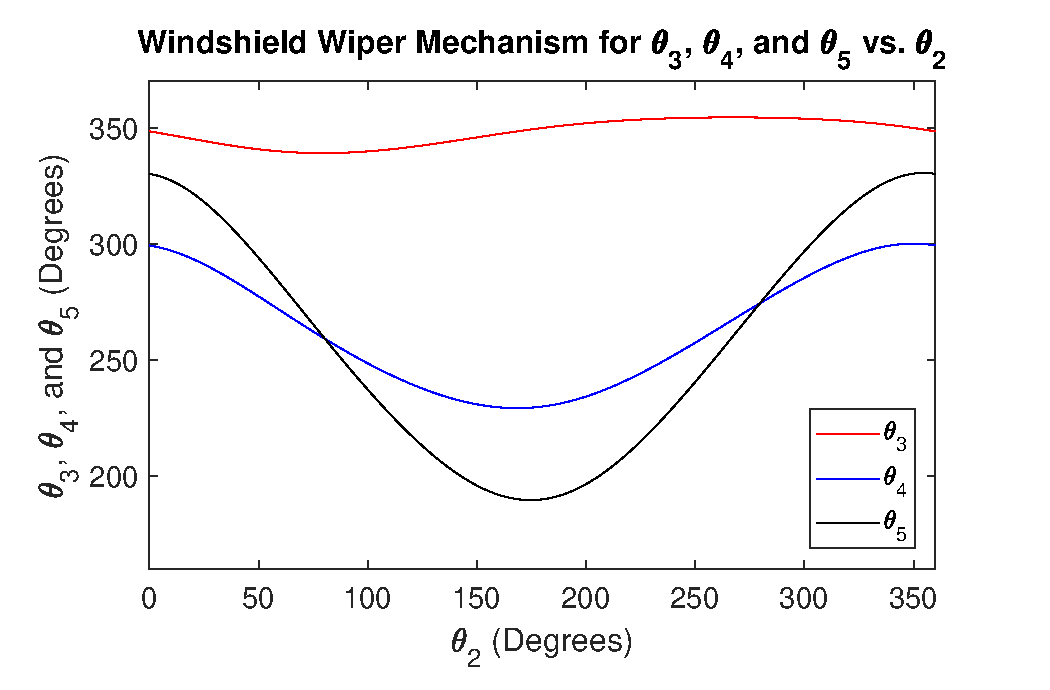
\includegraphics[width=5in]{figure1.eps}
  \end{array}$
  \end{center}
  \caption{Newton's Method approximation of a Windshield Wiper Mechanism displaying its trajectory of $\theta_3$, $\theta_4$, and $\theta_5$ with increasing $\theta_2$}
  \label{x4}
  \end{figure}
  \end{landscape}
  %%%%%%%%%%%%%%%%%%%%%%%%%%%%%%%%%%%%%%%%%%%%%%%%%%%%%%%%%%%%%%%%%%%%%%%%%%%%%%%%%%%%%%%%%%%
  \newpage
  %%%%%%%%%%%%%%%%%%%%%%%%%%%%%%%%%%%%%%%%%%%%%%%%%%%%%%%%%%%%%%%%%%%%%%%%%%%%%%%%%%%%%%%%%%%
  \begin{landscape}
  \begin{figure}[H]
  \begin{center}
  $\begin{array}{c}
  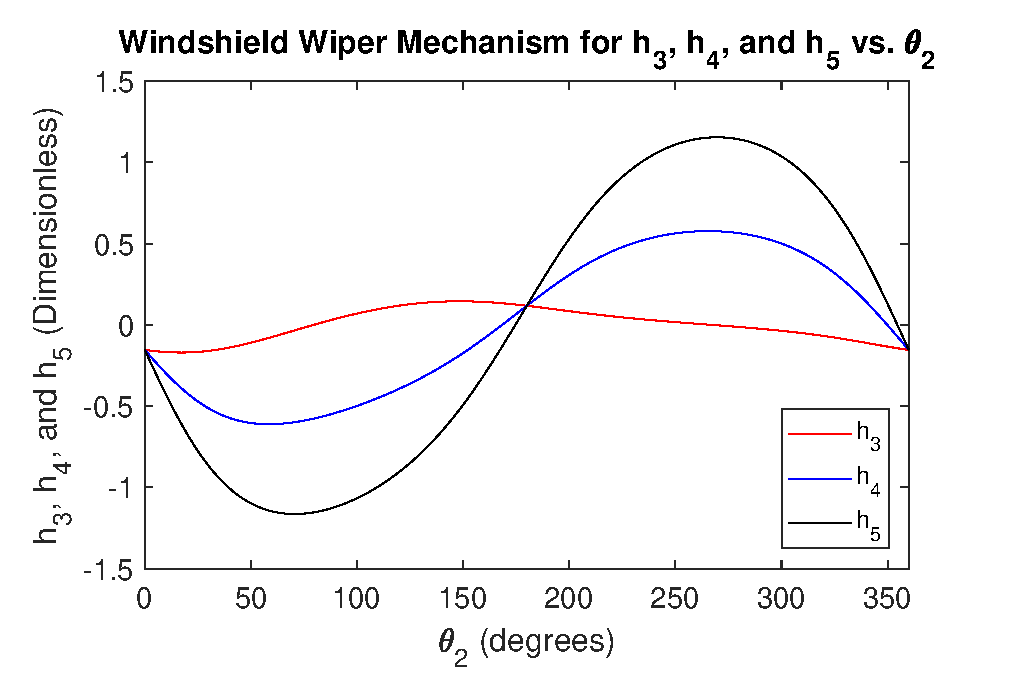
\includegraphics[width=5in]{figure2.eps}
  \end{array}$
  \end{center}
  \caption{Another Newton's Method approximation of a Windshield Wiper Mechanism displaying its trajectory of $1^{st}$ order Kinematic Coefficients with increasing $\theta_2$}
  \label{x5}
  \end{figure}
  \end{landscape}
  %%%%%%%%%%%%%%%%%%%%%%%%%%%%%%%%%%%%%%%%%%%%%%%%%%%%%%%%%%%%%%%%%%%%%%%%%%%%%%%%%%%%%%%%%%%
  \begin{landscape}
  \begin{figure}[H]
  \begin{center}
  $\begin{array}{c}
  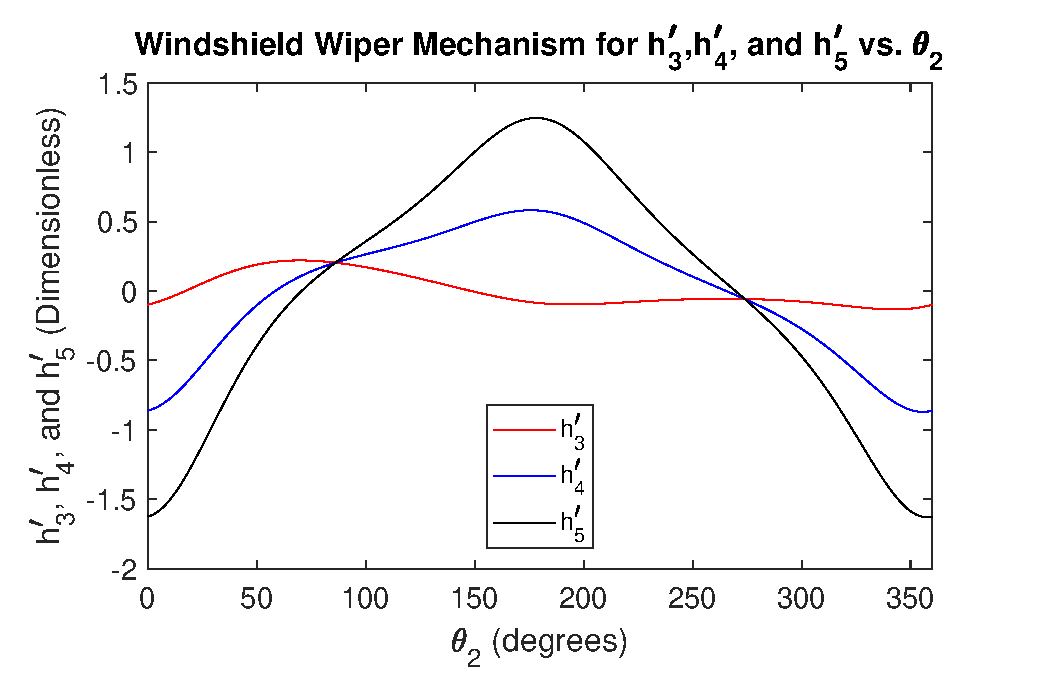
\includegraphics[width=5in]{figure3.eps}
  \end{array}$
  \end{center}
  \caption{Another Newton's Method approximation of a Windshield Wiper Mechanism displaying its trajectory of $2^{nd}$ order Kinematic Coefficients with increasing $\theta_2$}
  \label{x6}
  \end{figure}
  \end{landscape}
%%%%%%%%%%%%%%%%%%%%%%%%%%%%%%%%%%%%%%%%%%%%%%%%%%%%%%%%%%%%%%%%%%%%%%%%%%%%%%%%%%%%%%%%%%%%%%%
  \begin{landscape}
  \begin{figure}[H]
  \begin{center}
  $\begin{array}{c}
  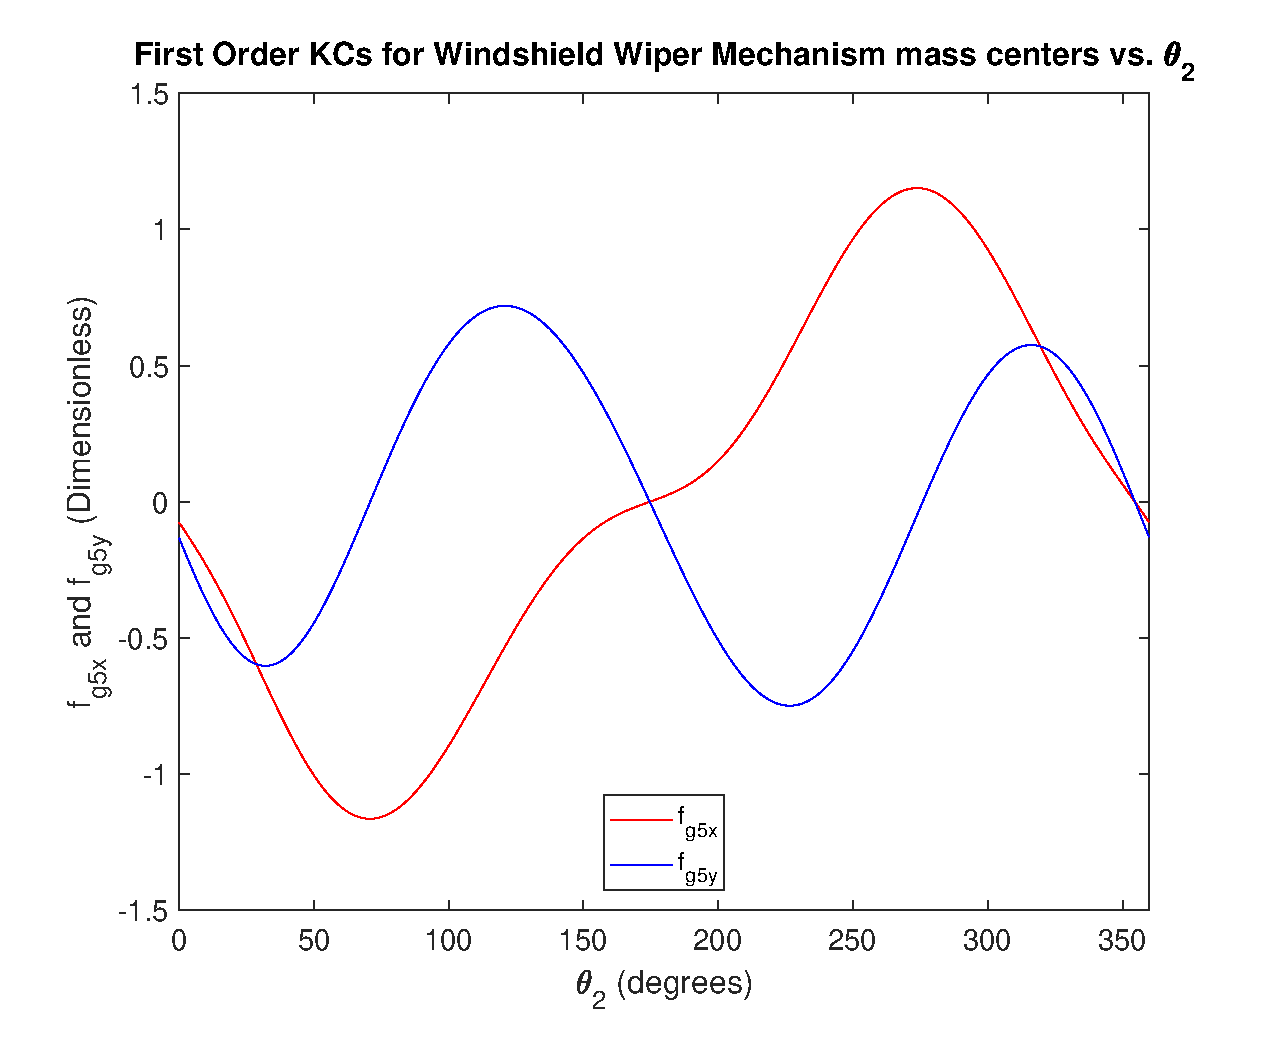
\includegraphics[width=5in]{figure4.eps}
  \end{array}$
  \end{center}
  \caption{Newton's Method approximation of a Windshield Wiper Blade of Function 2 displaying its trajectory of $1^{st}$ order Kinematic Coefficients with increasing $\theta_2$}
  \label{x7}
  \end{figure}
  \end{landscape}
  %%%%%%%%%%%%%%%%%%%%%%%%%%%%%%%%%%%%%%%%%%%%%%%%%%%%%%%%%%%%%%%%%%%%%%%%%%%%%%%%%%%%%%%%%%%
  \newpage
  %%%%%%%%%%%%%%%%%%%%%%%%%%%%%%%%%%%%%%%%%%%%%%%%%%%%%%%%%%%%%%%%%%%%%%%%%%%%%%%%%%%%%%%%%%%
  \begin{landscape}
  \begin{figure}[H]
  \begin{center}
  $\begin{array}{c}
  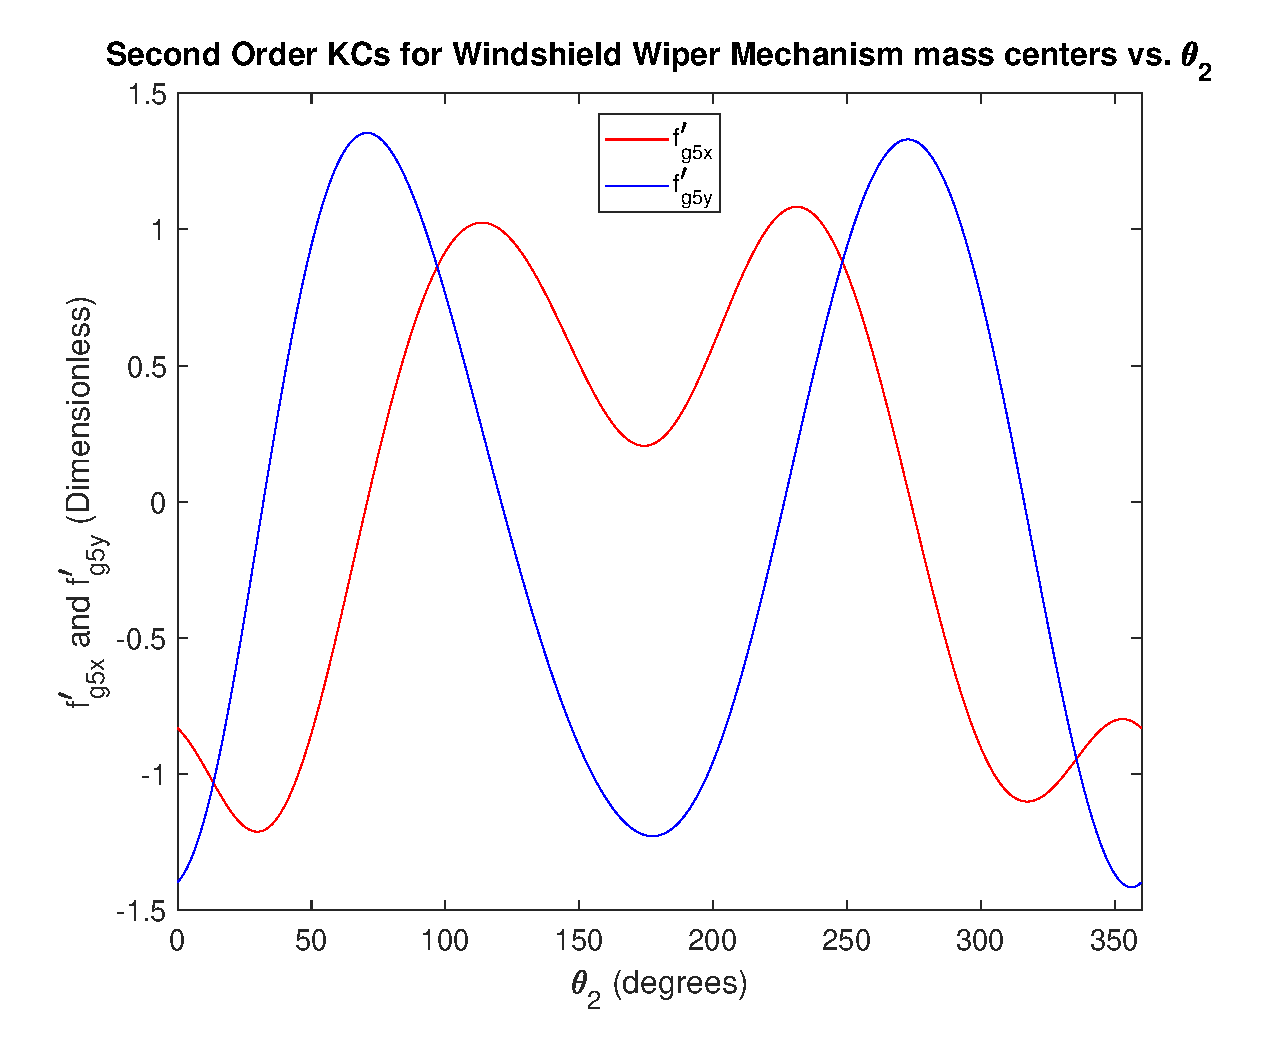
\includegraphics[width=5in]{figure5.eps}
  \end{array}$
  \end{center}
  \caption{Another Newton's Method approximation of a Windshield Wiper Blade of Function 2 displaying its trajectory of $1^{nd}$ order Kinematic Coefficients with increasing $\theta_2$}
  \label{x8}
  \end{figure}
  \end{landscape}
%%%%%%%%%%%%%%%%%%%%%%%%%%%%%%%%%%%%%%%%%%%%%%%%%%%%%%%%%%%%%%%%%%%%%%%%%%%%%%%%%%%%%%%%%%%%%%
  \begin{landscape}
  \begin{figure}[H]
  \begin{center}
  $\begin{array}{c}
  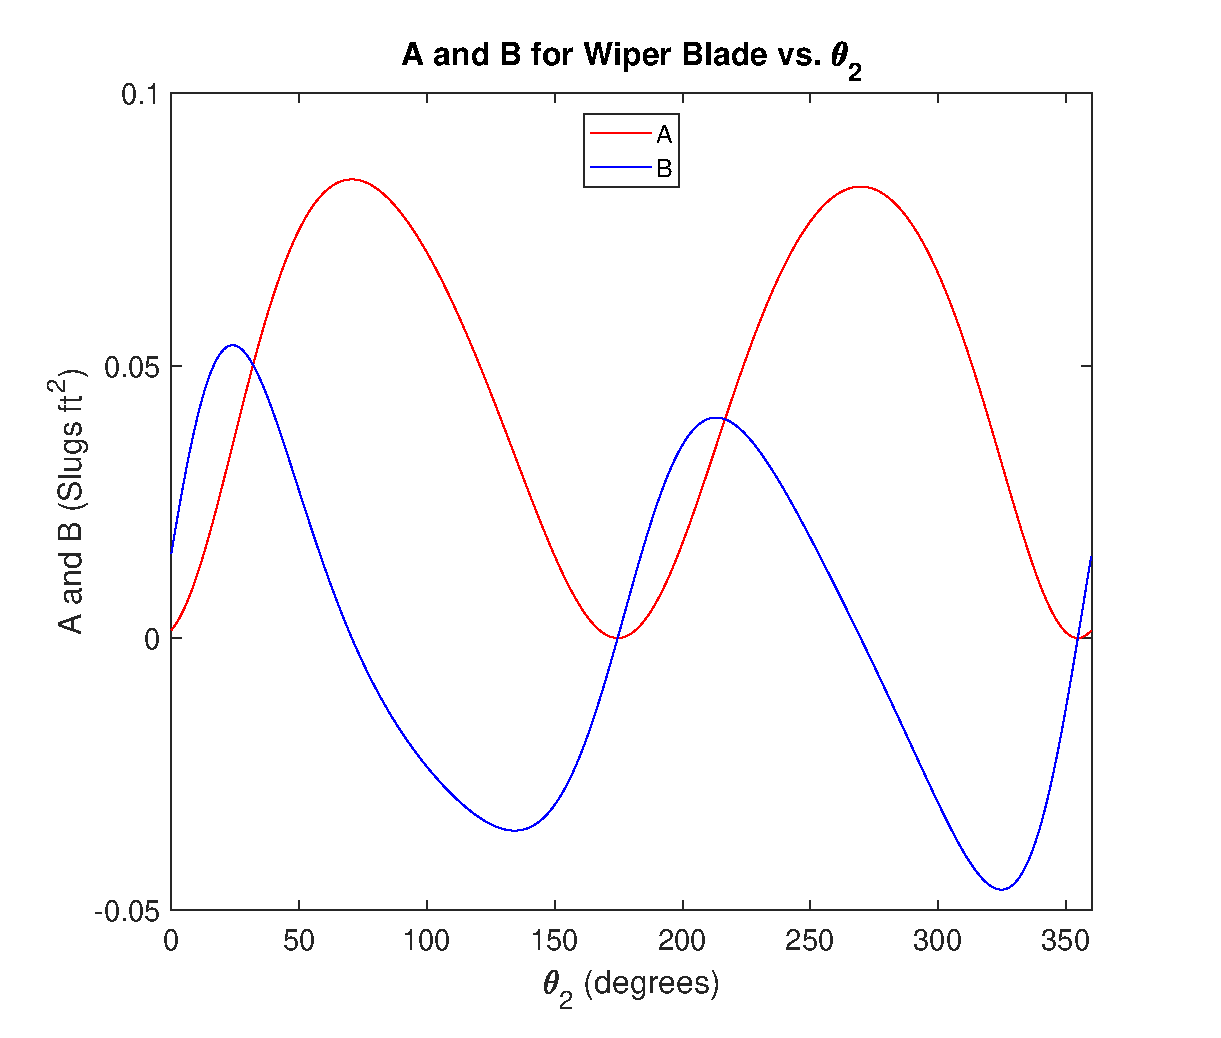
\includegraphics[width=5in]{figure6.eps}
  \end{array}$
  \end{center}
  \caption{Approximation of rate of change of kinetic energy for a Windshield Wiper Blade of Function 3 describing the motion of moving parts within the machine with increasing $\theta_2$}
  \label{x9}
  \end{figure}
  \end{landscape}
  %%%%%%%%%%%%%%%%%%%%%%%%%%%%%%%%%%%%%%%%%%%%%%%%%%%%%%%%%%%%%%%%%%%%%%%%%%%%%%%%%%%%%%%%%%%
  \newpage
  %%%%%%%%%%%%%%%%%%%%%%%%%%%%%%%%%%%%%%%%%%%%%%%%%%%%%%%%%%%%%%%%%%%%%%%%%%%%%%%%%%%%%%%%%%%
  \begin{landscape}
  \begin{figure}[H]
  \begin{center}
  $\begin{array}{c}
  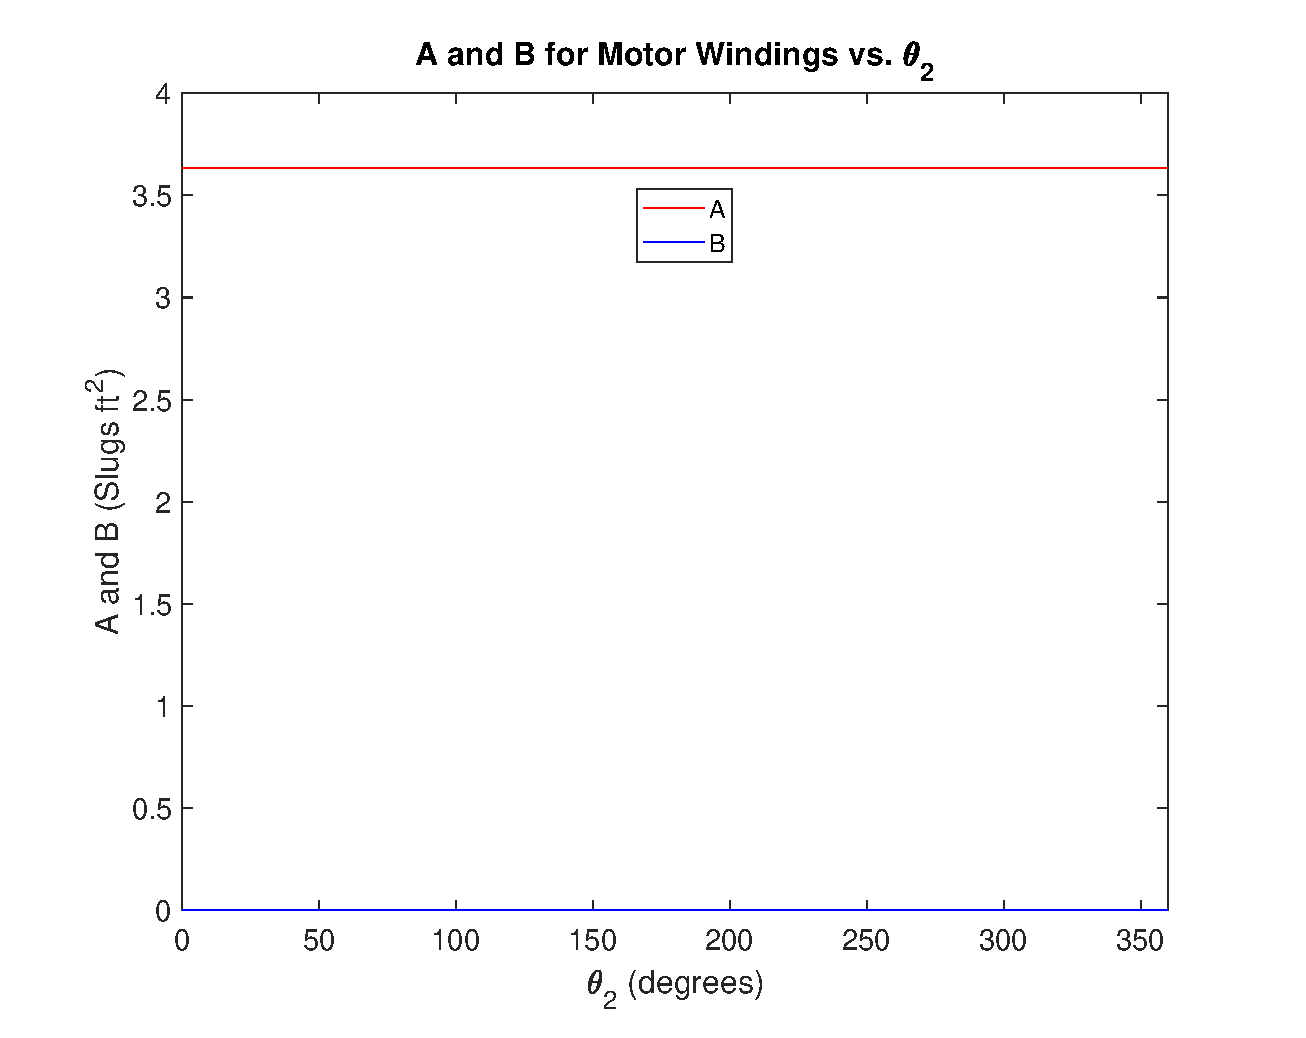
\includegraphics[width=5in]{figure7.eps}
  \end{array}$
  \end{center}
  \caption{Rate of change of kinetic energy analysis for Motor Windings of Function 3 describing the motion of moving parts within the machine with increasing $\theta_2$}
  \label{x10}
  \end{figure}
  \end{landscape}
  %%%%%%%%%%%%%%%%%%%%%%%%%%%%%%%%%%%%%%%%%%%%%%%%%%%%%%%%%%%%%%%%%%%%%%%%%%%%%%%%%%%%%%%%%%%
    \newpage
  %%%%%%%%%%%%%%%%%%%%%%%%%%%%%%%%%%%%%%%%%%%%%%%%%%%%%%%%%%%%%%%%%%%%%%%%%%%%%%%%%%%%%%%%%%%
  \begin{landscape}
  \begin{figure}[H]
  \begin{center}
  $\begin{array}{c}
  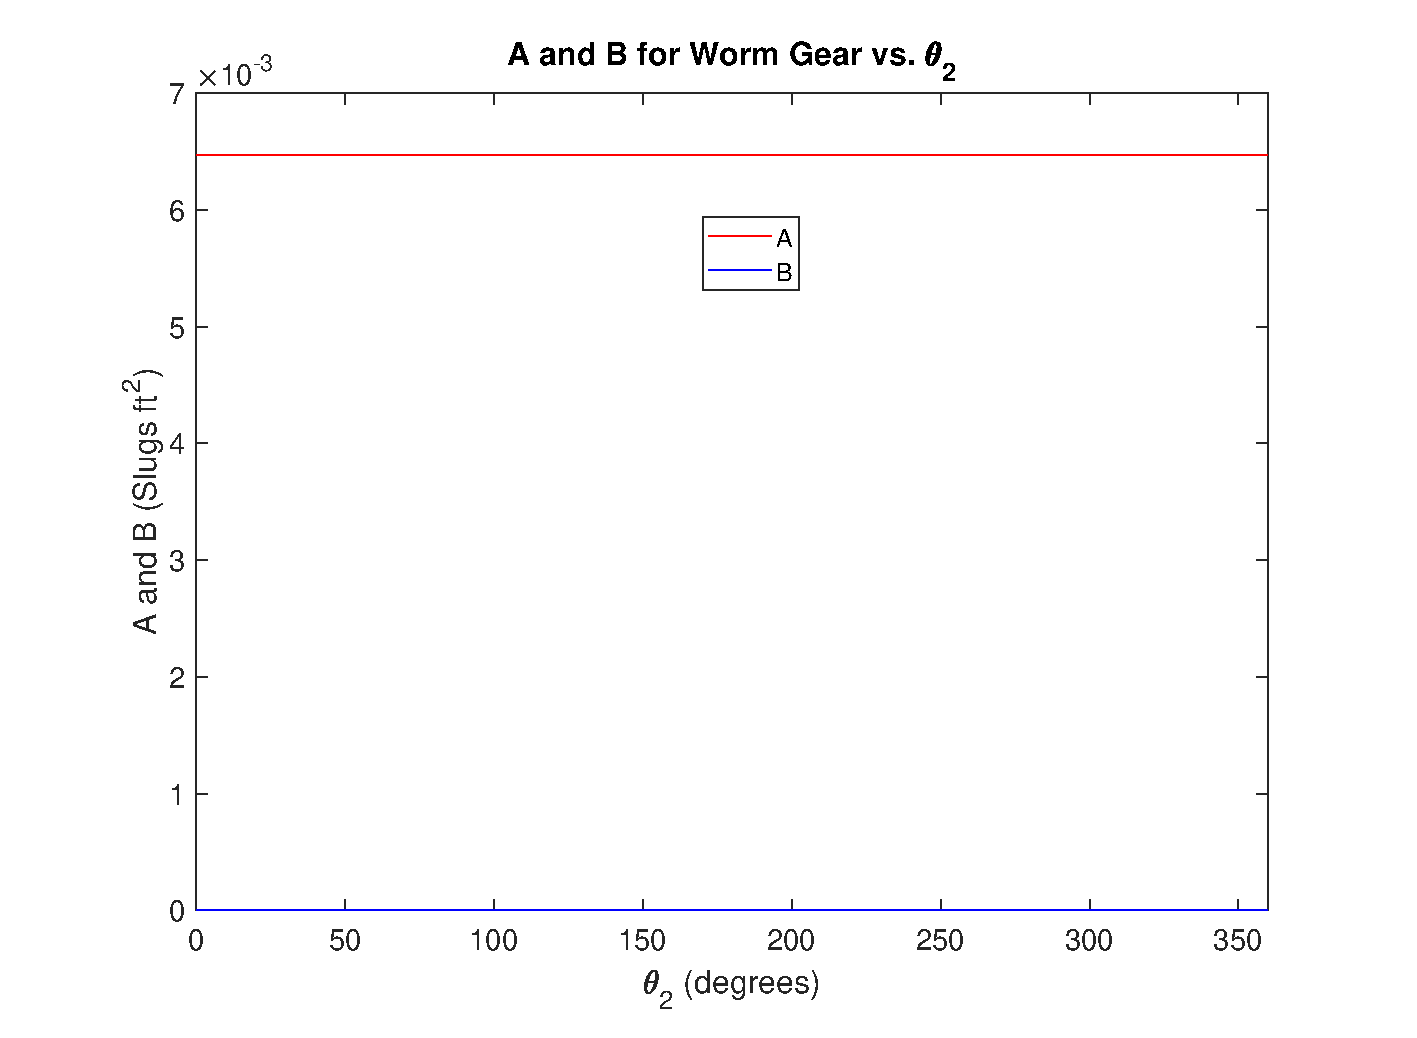
\includegraphics[width=5in]{figure8.eps}
  \end{array}$
  \end{center}
  \caption{Rate of change of kinetic energy analysis for Worm Gear of Function 3 describing the motion of moving parts within the machine with increasing $\theta_2$}
  \label{x11}
  \end{figure}
  \end{landscape}
  %%%%%%%%%%%%%%%%%%%%%%%%%%%%%%%%%%%%%%%%%%%%%%%%%%%%%%%%%%%%%%%%%%%%%%%%%%%%%%%%%%%%%%%%%%%%%
  \newpage
  %%%%%%%%%%%%%%%%%%%%%%%%%%%%%%%%%%%%%%%%%%%%%%%%%%%%%%%%%%%%%%%%%%%%%%%%%%%%%%%%%%%%%%%%%%%
  \begin{landscape}
  \begin{figure}[H]
  \begin{center}
  $\begin{array}{c}
  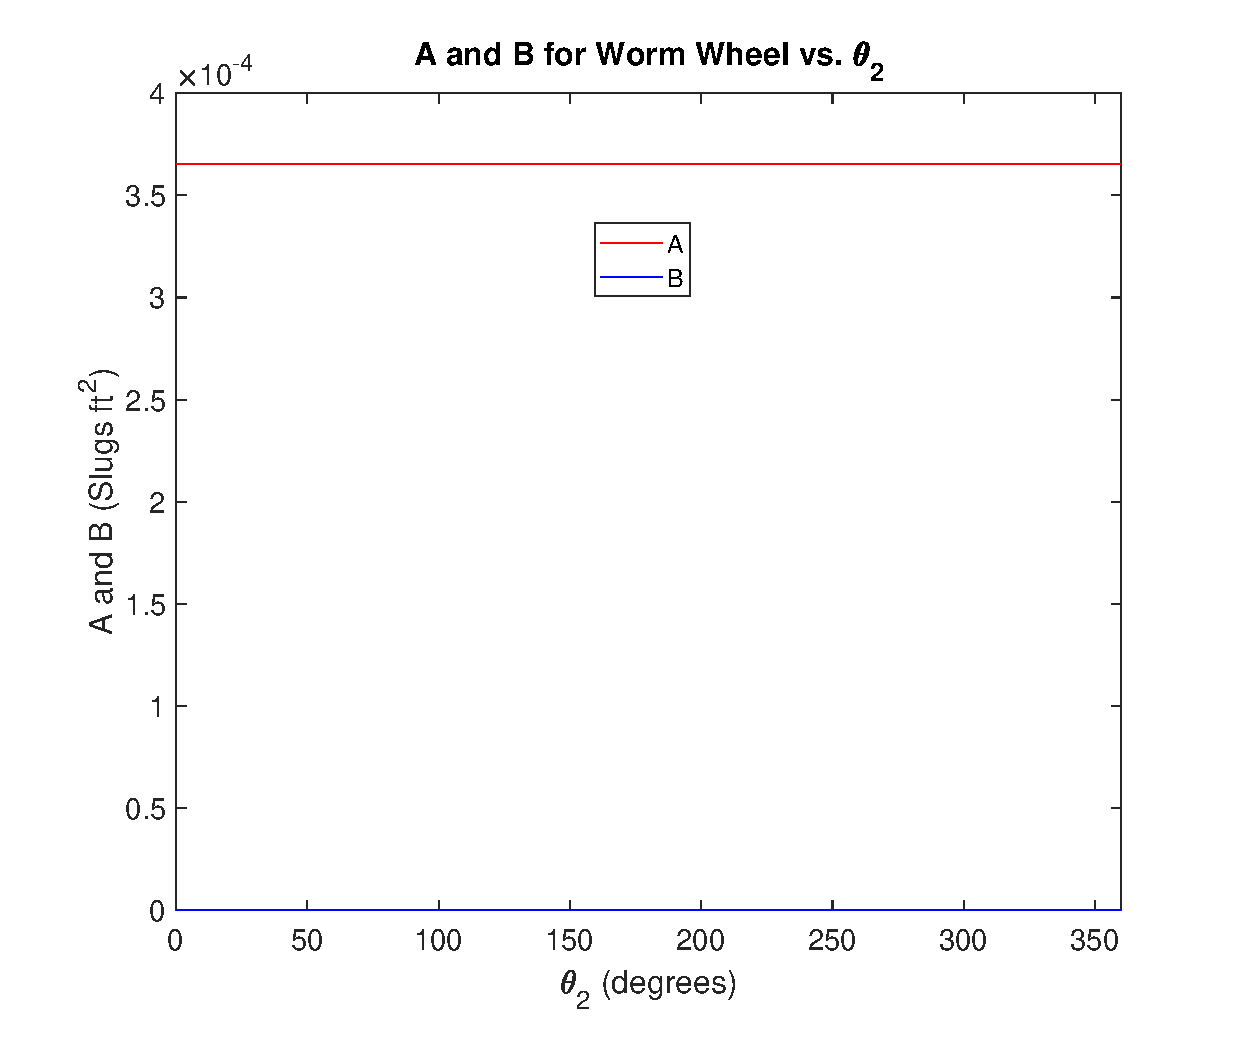
\includegraphics[width=5in]{figure9.eps}
  \end{array}$
  \end{center}
  \caption{Rate of change of kinetic energy analysis for Worm Wheel of Function 3 describing the motion of moving parts within the machine with increasing $\theta_2$}
  \label{x12}
  \end{figure}
  \end{landscape}
  %%%%%%%%%%%%%%%%%%%%%%%%%%%%%%%%%%%%%%%%%%%%%%%%%%%%%%%%%%%%%%%%%%%%%%%%%%%%%%%%%%%%%%%%%%%%%
  \newpage
  %%%%%%%%%%%%%%%%%%%%%%%%%%%%%%%%%%%%%%%%%%%%%%%%%%%%%%%%%%%%%%%%%%%%%%%%%%%%%%%%%%%%%%%%%%%
  \begin{landscape}
  \begin{figure}[H]
  \begin{center}
  $\begin{array}{c}
  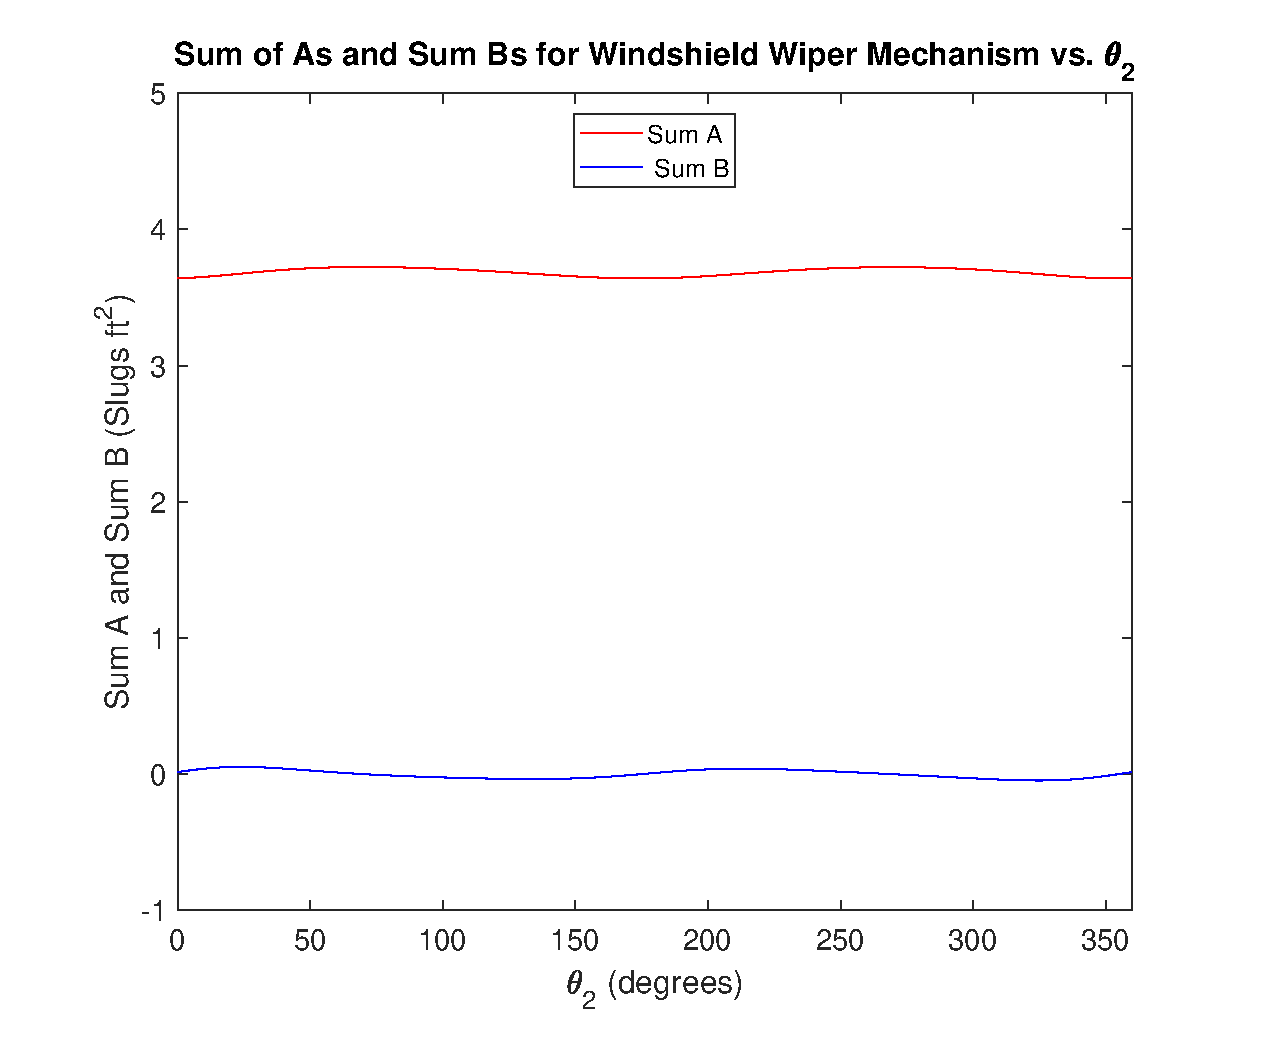
\includegraphics[width=5in]{figure10.eps}
  \end{array}$
  \end{center}
  \caption{Rate of change of kinetic energy summation for the WindShield Wiper Mechanism of Function 3 describing the motion of moving parts within the machine with increasing $\theta_2$}
  \label{x13}
  \end{figure}
  \end{landscape}
%%%%%%%%%%%%%%%%%%%%%%%%%%%%%%%%%%%%%%%%%%%%%%%%%%%%%%%%%%%%%%%%%%%%%%%%%%%%%%%%%%%%%%%%%%%%%%%
  \begin{landscape}
  \begin{figure}[H]
  \begin{center}
  $\begin{array}{c}
  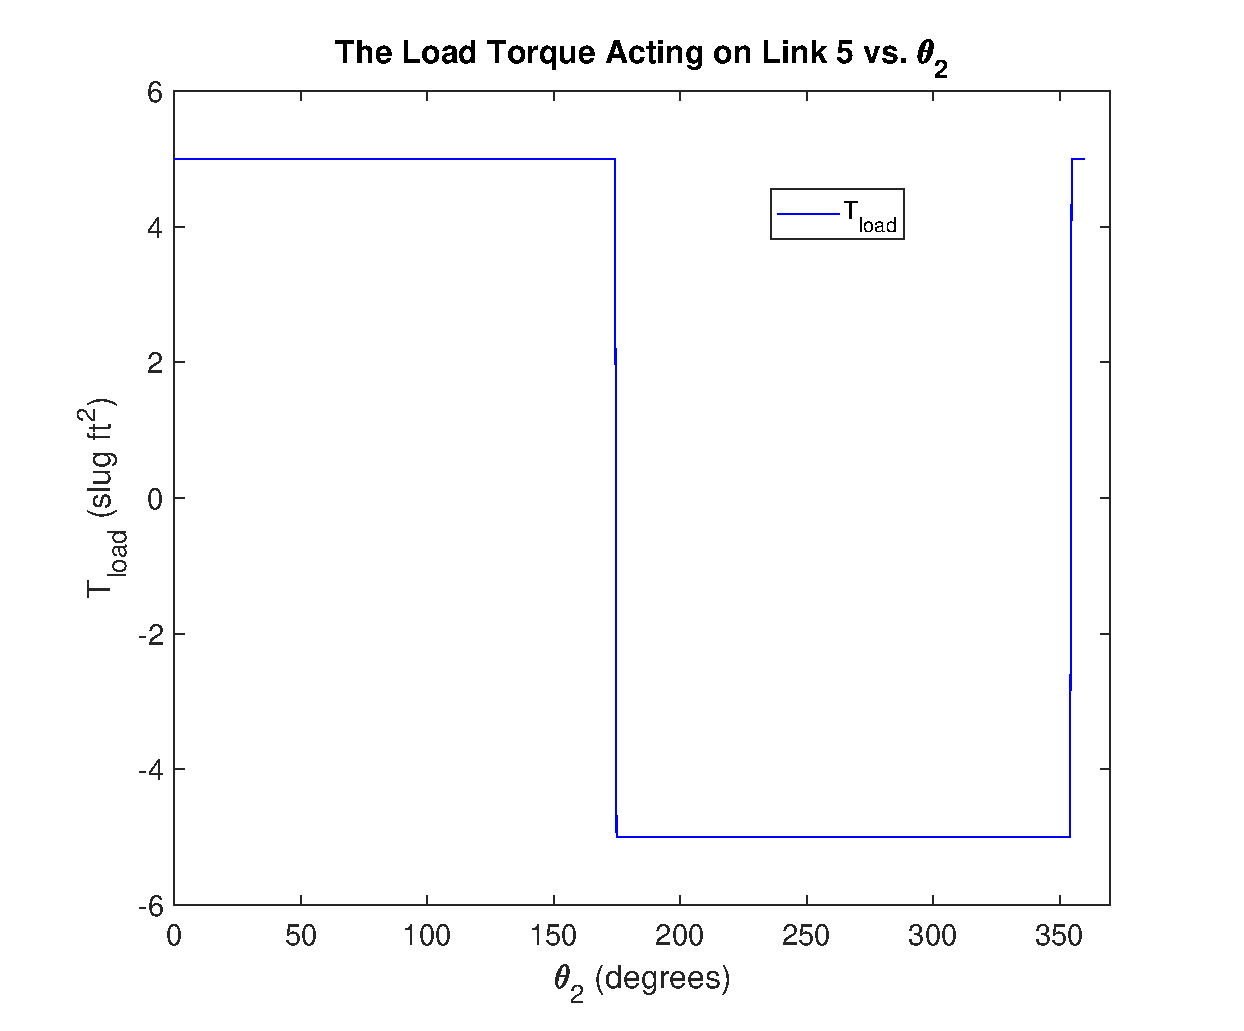
\includegraphics[width=5in]{figure11.eps}
  \end{array}$
  \end{center}
  \caption{Graphical representation of an Inverse Dynamics Problem of Function 4 applied to motor selection AM238 Series gearmotor outputting the load torque acting on link 5 with increasing $\theta_2$}
  \label{x14}
  \end{figure}
  \end{landscape}
  %%%%%%%%%%%%%%%%%%%%%%%%%%%%%%%%%%%%%%%%%%%%%%%%%%%%%%%%%%%%%%%%%%%%%%%%%%%%%%%%%%%%%%%%%%%%%
  \newpage
  %%%%%%%%%%%%%%%%%%%%%%%%%%%%%%%%%%%%%%%%%%%%%%%%%%%%%%%%%%%%%%%%%%%%%%%%%%%%%%%%%%%%%%%%%%%
  \begin{landscape}
  \begin{figure}[H]
  \begin{center}
  $\begin{array}{c}
  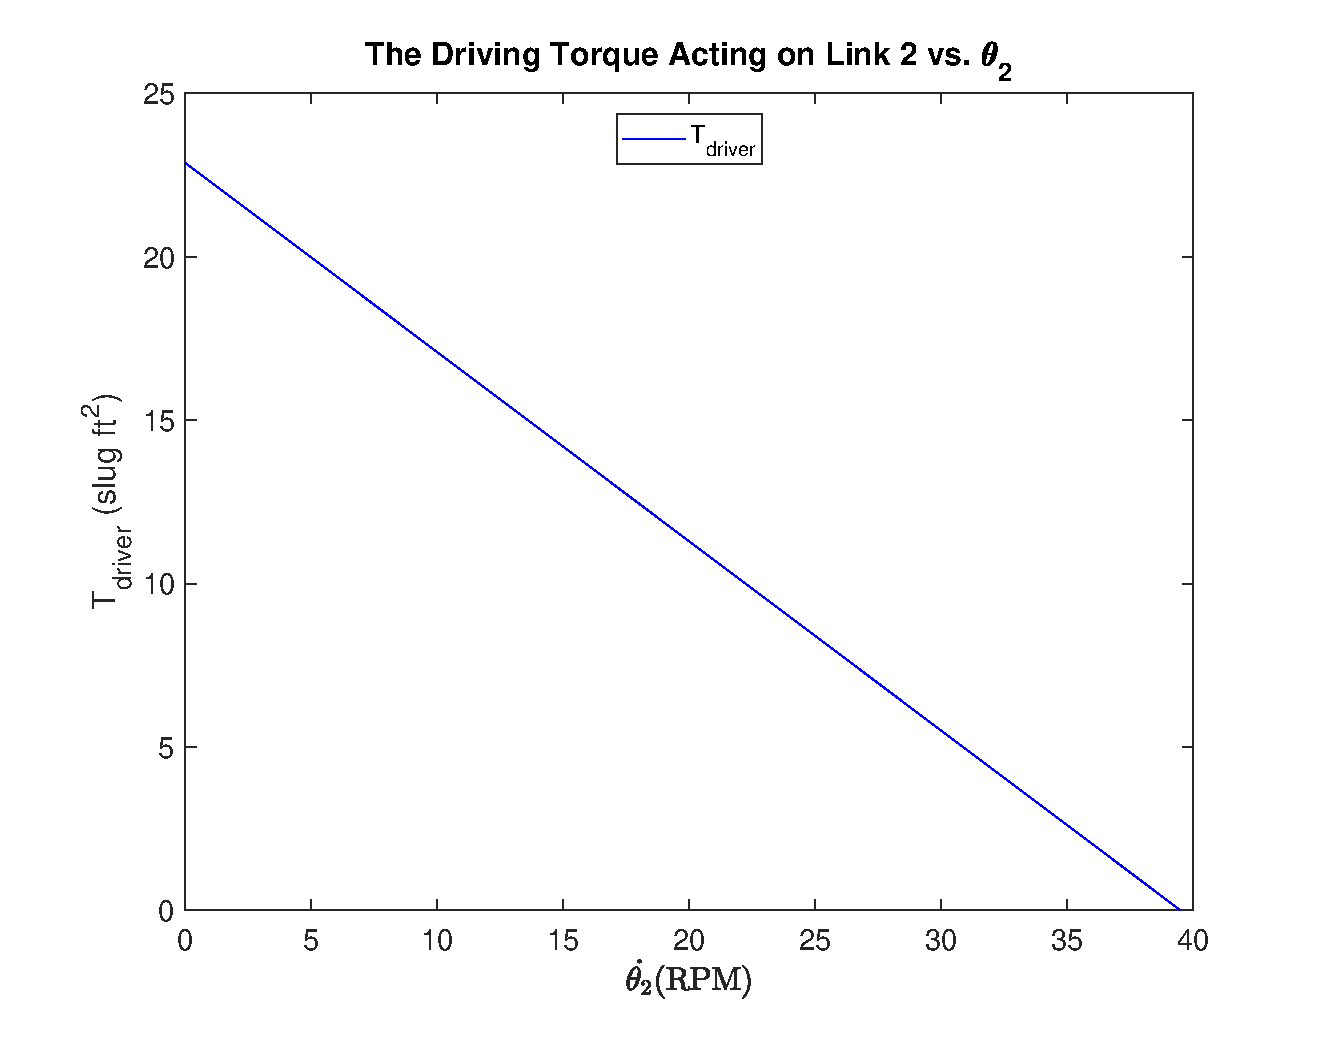
\includegraphics[width=5in]{figure12.eps}
  \end{array}$
  \end{center}
  \caption{Velocity rate of change of joint variable $\dot{\theta_2}$ in revolutions per minute of Function 5 describing the driving torque acting on link 2}
  \label{x15}
  \end{figure}
  \end{landscape}
%%%%%%%%%%%%%%%%%%%%%%%%%%%%%%%%%%%%%%%%%%%%%%%%%%%%%%%%%%%%%%%%%%%%%%%%%%%%%%%%%%%%%%%%%%%%
\section*{Appendix J}

%This section shows the specifications of the AM equipment 238 motor.

  \begin{figure}[H]
  \begin{center}
  $\begin{array}{c}
  \includegraphics[width=6.5in]{wiper1.pdf}
  \end{array}$
  \end{center}
  \caption{AM equipment 238 motor specifications front}
  \label{x16}
  \end{figure}
%%%%%%%%%%%%%%%%%%%%%%%%%%%%%%%%%%%%%%%%%%%%%%%%%%%%%%%%%%%%%%%%%%%%%%%%%%%%%%%%%%%%%%%%%%
  \begin{figure}[H]
  \begin{center}
  $\begin{array}{c}
  \includegraphics[width=6.5in]{wiper2.pdf}
  \end{array}$
  \end{center}
  \caption{AM equipment 238 motor specifications back}
  \label{x17}
  \end{figure}
%%%%%%%%%%%%%%%%%%%%%%%%%%%%%%%%%%%%%%%%%%%%%%%%%%%%%%%%%%%%%%%%%%%%%%%%%%%%%%%%%%%%%%%%%%%%
\end{document}